%60
\subsection{Új elem beillesztése adott elem után}
\begin{frame}
  \begin{columns}[c]
    \column{0.5\textwidth}
      \scriptsize
      \begin{exampleblock}{\textattachfile{Lista2.cpp}{Lista2.cpp}}
        \vspace{-.2cm}
        \lstinputlisting[style=cpp,linerange={4-20},numbers=left,firstnumber=4]{Lista2.cpp}
        \vspace{-.2cm}
    \end{exampleblock}
    \column{0.45\textwidth}
      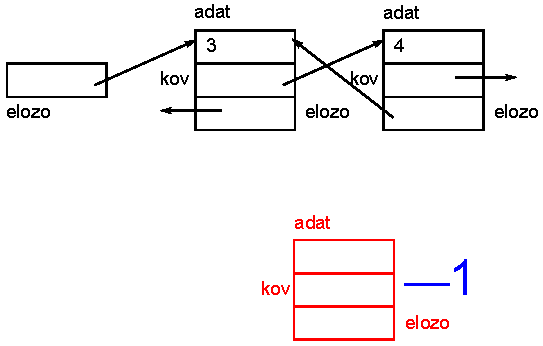
\includegraphics[width=\textwidth]{lista2/list2-1.pdf}
  \end{columns}
\end{frame}

%61
\begin{frame}
  \begin{columns}[c]
    \column{0.5\textwidth}
      \scriptsize
      \begin{exampleblock}{\textattachfile{Lista2.cpp}{Lista2.cpp}}
        \vspace{-.2cm}
        \lstinputlisting[style=cpp,linerange={4-20},numbers=left,firstnumber=4]{Lista2.cpp}
        \vspace{-.2cm}
    \end{exampleblock}
    \column{0.45\textwidth}
      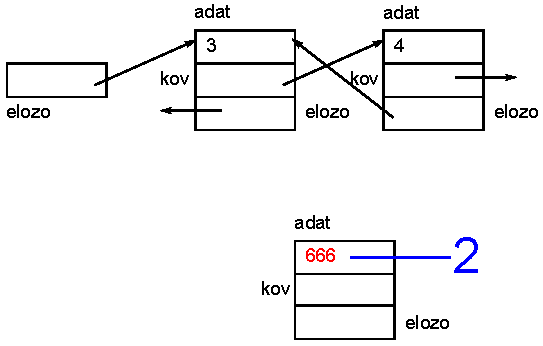
\includegraphics[width=\textwidth]{lista2/list2-2.pdf}
  \end{columns}
\end{frame}

%62
\begin{frame}
  \begin{columns}[c]
    \column{0.5\textwidth}
      \scriptsize
      \begin{exampleblock}{\textattachfile{Lista2.cpp}{Lista2.cpp}}
        \vspace{-.2cm}
        \lstinputlisting[style=cpp,linerange={4-20},numbers=left,firstnumber=4]{Lista2.cpp}
        \vspace{-.2cm}
    \end{exampleblock}
    \column{0.45\textwidth}
      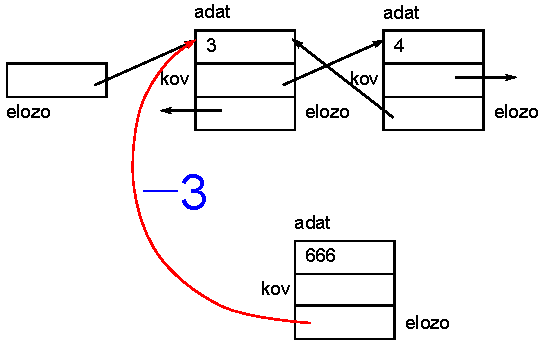
\includegraphics[width=\textwidth]{lista2/list2-3.pdf}
  \end{columns}
\end{frame}

%63
\begin{frame}
  \begin{columns}[c]
    \column{0.5\textwidth}
      \scriptsize
      \begin{exampleblock}{\textattachfile{Lista2.cpp}{Lista2.cpp}}
        \vspace{-.2cm}
        \lstinputlisting[style=cpp,linerange={4-20},numbers=left,firstnumber=4]{Lista2.cpp}
        \vspace{-.2cm}
    \end{exampleblock}
    \column{0.45\textwidth}
      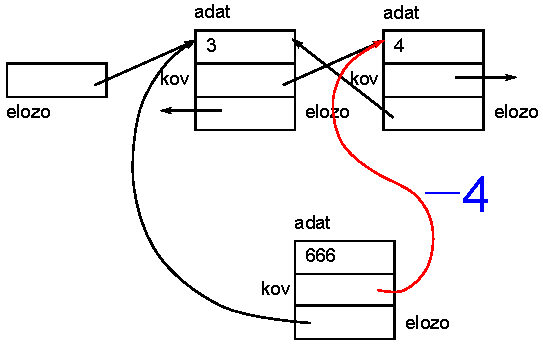
\includegraphics[width=\textwidth]{lista2/list2-4.pdf}
  \end{columns}
\end{frame}

%64
\begin{frame}
  \begin{columns}[c]
    \column{0.5\textwidth}
      \scriptsize
      \begin{exampleblock}{\textattachfile{Lista2.cpp}{Lista2.cpp}}
        \vspace{-.2cm}
        \lstinputlisting[style=cpp,linerange={4-20},numbers=left,firstnumber=4]{Lista2.cpp}
        \vspace{-.2cm}
    \end{exampleblock}
    \column{0.45\textwidth}
      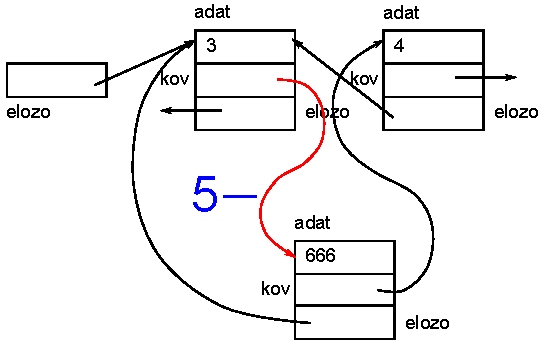
\includegraphics[width=\textwidth]{lista2/list2-5.pdf}
  \end{columns}
\end{frame}

%65
\begin{frame}
  \begin{columns}[c]
    \column{0.5\textwidth}
      \scriptsize
      \begin{exampleblock}{\textattachfile{Lista2.cpp}{Lista2.cpp}}
        \vspace{-.2cm}
        \lstinputlisting[style=cpp,linerange={4-20},numbers=left,firstnumber=4]{Lista2.cpp}
        \vspace{-.2cm}
    \end{exampleblock}
    \column{0.45\textwidth}
      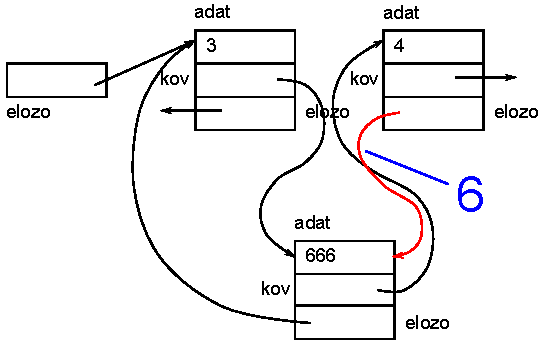
\includegraphics[width=\textwidth]{lista2/list2-6.pdf}
  \end{columns}
\end{frame}